\begin{frame}{Graphs}

\begin{columns}[T,onlytextwidth]
    \hspace{2em}
	\begin{column}{0.5\textwidth}
		\centering
        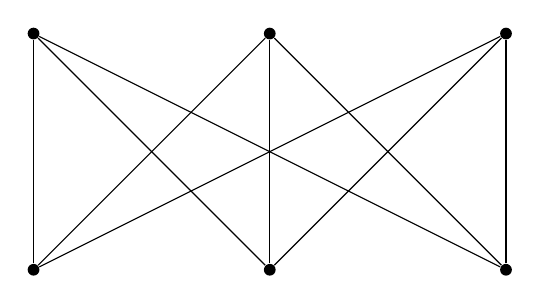
\begin{tikzpicture}[scale=3]
            \node[circle, fill, inner sep=1.5pt] (v1) at (0,0) {};
            \node[circle, fill, inner sep=1.5pt] (v2) at (1,0) {};
            \node[circle, fill, inner sep=1.5pt] (v3) at (2,0) {};
            \node[circle, fill, inner sep=1.5pt] (w1) at (0,1) {};
            \node[circle, fill, inner sep=1.5pt] (w2) at (1,1) {};
            \node[circle, fill, inner sep=1.5pt] (w3) at (2,1) {};
            \draw (v1) -- (w1);
            \draw (v1) -- (w2);
            \draw (v1) -- (w3);
            \draw (v2) -- (w1);
            \draw (v2) -- (w2);
            \draw (v2) -- (w3);
            \draw (v3) -- (w1);
            \draw (v3) -- (w2);
            \draw (v3) -- (w3);

        \end{tikzpicture}
        
        \vspace{1em}
		\scriptsize \(K_{3,3}\)
	\end{column}

	\begin{column}{0.5\textwidth}
		\centering
        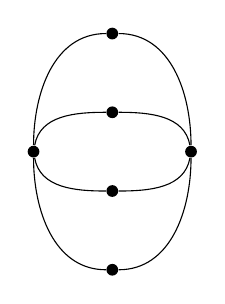
\begin{tikzpicture}[scale=1]

            % Define the two main suspension vertices, positioned closer together
            \node[circle, fill, inner sep=1.5pt] (a1) at (0,0) {};
            \node[circle, fill, inner sep=1.5pt] (a2) at (2,0) {};

            \node[circle, fill, inner sep=1.5pt] (b1) at (1,1.5) {};
            \node[circle, fill, inner sep=1.5pt] (b2) at (1,.5) {};
            \node[circle, fill, inner sep=1.5pt] (b3) at (1,-.5) {};
            \node[circle, fill, inner sep=1.5pt] (b4) at (1,-1.5) {};


    % Draw the edges for the 'm' paths, passing through the b_i nodes
    \draw (a1) to[out=90, in=180] (b1);
    \draw (a1) to[out=80, in=180] (b2);
    \draw (a1) to[out=-80, in=180] (b3);
    \draw (a1) to[out=-90, in=180] (b4);

    \draw (a2) to[out=90, in=0] (b1);
    \draw (a2) to[out=100, in=0] (b2);
    \draw (a2) to[out=-100, in=0] (b3);
    \draw (a2) to[out=-90, in=0] (b4);

        \end{tikzpicture}

        \vspace{1em}
		\scriptsize \(K_{2,4}\)
    \end{column}
\end{columns}
\end{frame}